\section{Performance}

\figref{performanceNorm} together with the statistical data in table \ref{score2} showed that there is a statistical difference in performance when controlling the ROV with and without predictive help. In addition, the effect size of $0.735$ can be categorized as a medium to large effect. Especially when considering how easy and cheap this predictive method is to implement. The subjects performed on average 20\% better. This can be a valuable increase in situations were performance degradation due to communication latency is a problem. With this in mind, H1, that a simple predictor display based on image transformation can increase the operator performance, is therefore verified.

Past research, table \ref{reviewPred}, describes a wide range performance gains from predictive technology. Everything from 8\% to 65\%. It's hard to do a direct comparison to any specific experiment, but a performance increase of 20\% in this experiment is probably in the lower range of what have been found before. What is true though, is that the predictive method described in this thesis is the cheapest and easiest to implement. This holds true when comparing to the experiments in the mentioned table.

None of the subjects were told that there would be a predictive display or how it worked. Some of the participants immediately identified what the predictive display was trying to tell them. Others however, didn't understand that there had been a predictive display until the experiment was over. The ones who tried to use the predictive display the way it was intended typically performed better than those who didn't. It may be possible that we could have seen an improved performance, if the subjects were informed how the predictive display works. This can however not be verified unless additional experiments are performed.

It is also interesting the evaluate if participants had any learning effects during the experiment. \figref{learning_effect} shows the score for each display type and further divided into groups depending on the subject had that display as the first, second or third display. As an example, the first of the nine box plots describes the score achieved in the delay condition for those who had that display as their first display. One visible trend is that the participants who had a particular display as their second display, performed better than those who had that display as their first. This performance increase was significant for all displays. Delay: t(18)=2.19, p=0.042, d=0.671, delay PD: t(17)=2.19, p=0.043, d=0.660, no delay: t(17)=3.26, p=0.005, d=0.902. The performance change from \#2 to \#3 in all displays were however not found significant.

\begin{figure}[h!]
    \centering
    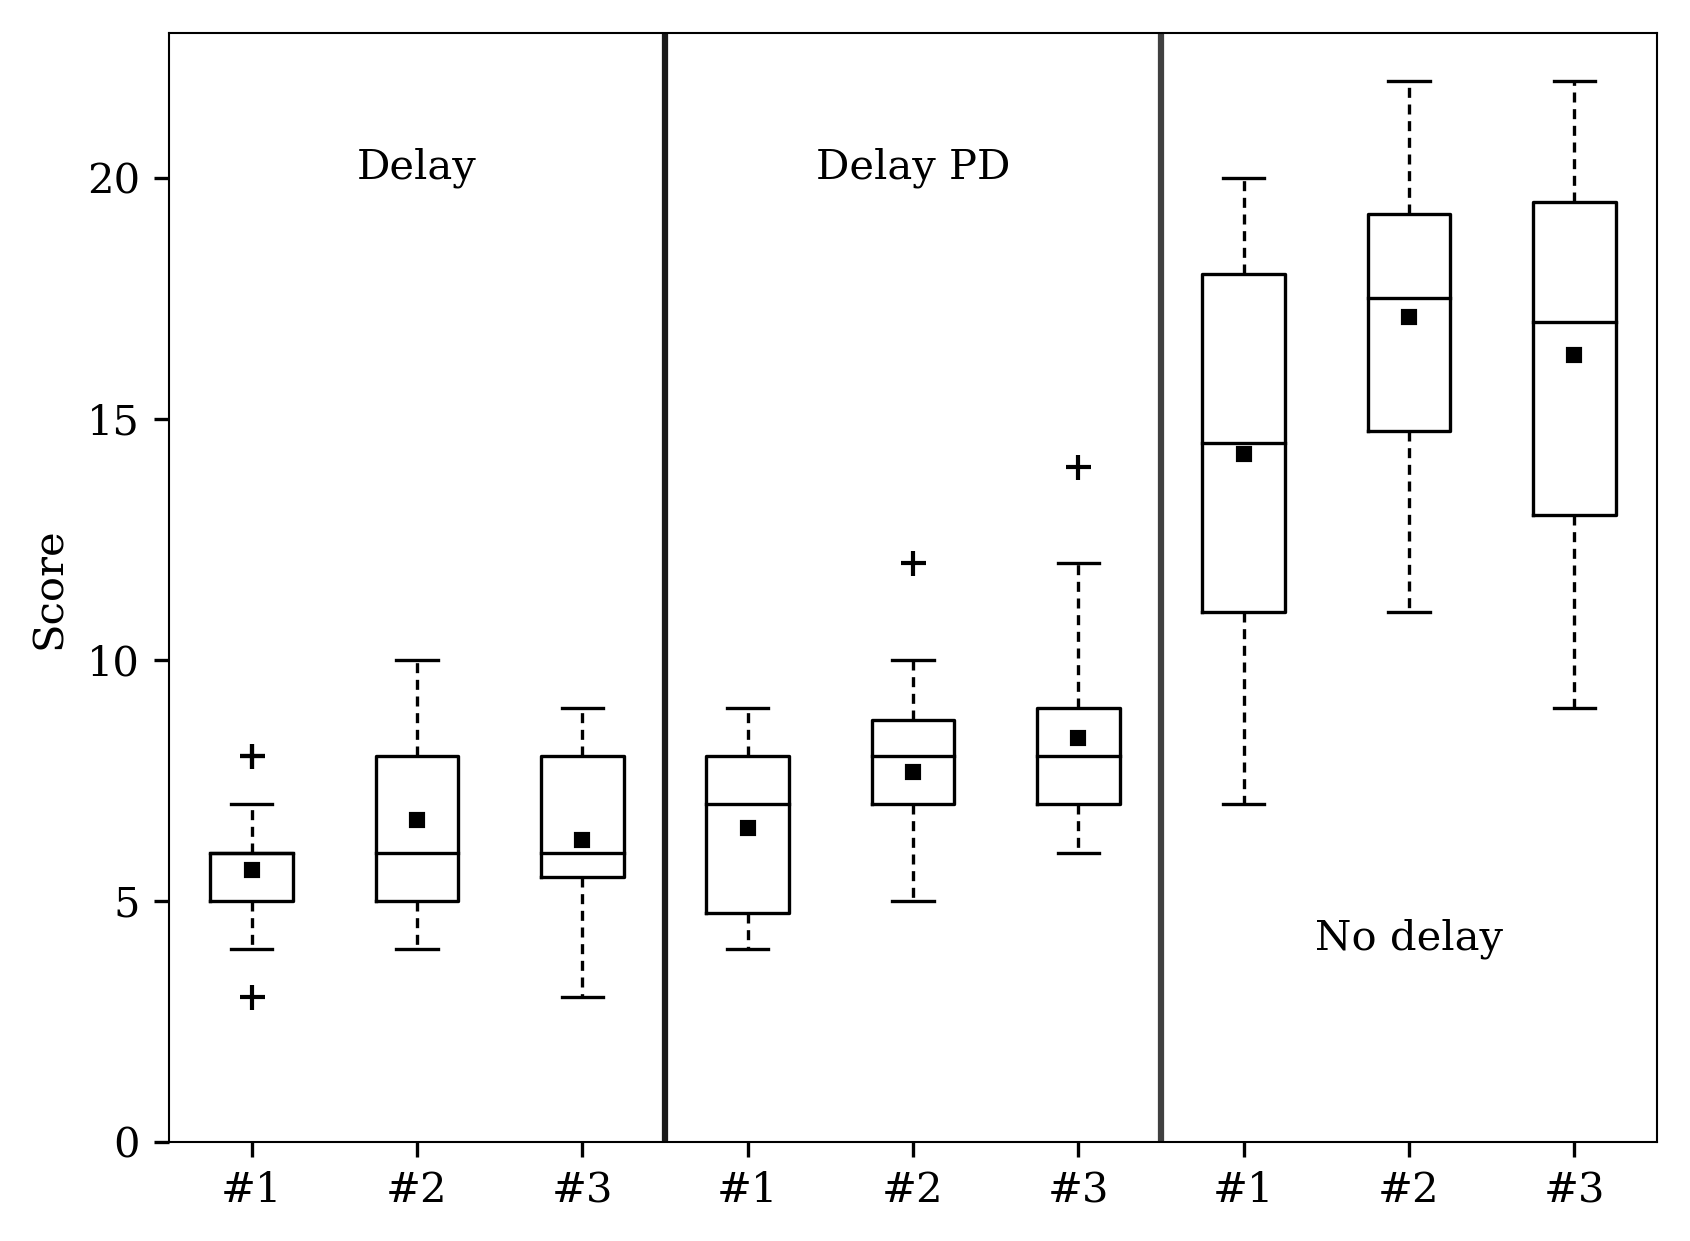
\includegraphics[width=0.7\textwidth]{learning_effect}
    \caption{Score categorized after display order.}
    \label{learning_effect}
\end{figure}

The participants were also asked how much computer games the play. \figref{gamer_performance} shows the score in each display type for gamer (G), versus non gamer (NG). Gamers are defined as those who play video games weekly or more and they made up 30\% of the total experiment group. It is interesting to see that G's only performed better than NG's when using predictive or no delay display. PD: t(26.57)=2.23, p=0.034, d=0.692 and no delay: t(40.79)=2.56, p=0.014, d=0.660.

By looking at the performance difference between a delayed display without and with predictive technology. It also becomes clear that gamers had a bigger gain using the predictive display. While NG's had a moderate effect size of 0.577, t(39)=3.27, p=0.002, d=0.577. Gamers had almost twice the effect size of 1.018, t(16)=4.17, $p<.001$, d=1.018. Exactly why G's were able to increase their performance more using the PD is unclear. It could be that the arrow in the PD which acts like an aiming device, is a more familiar concept for gamers.


\begin{figure}[h!]
    \centering
    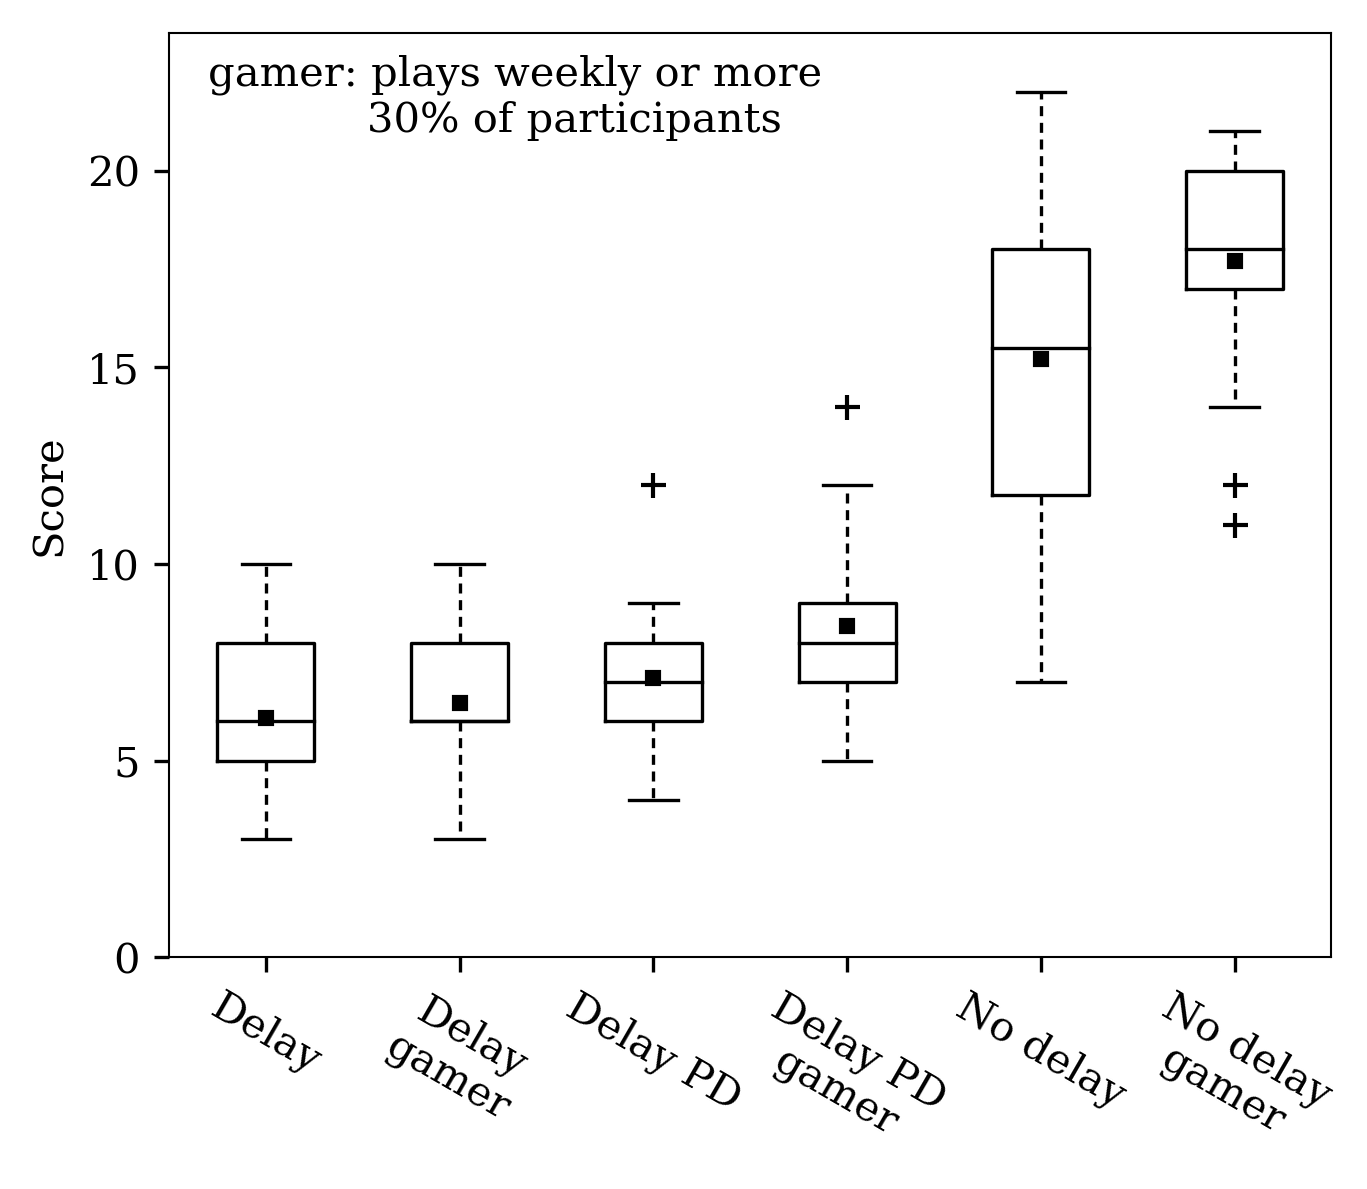
\includegraphics[scale=0.85]{gamer_performance}
    \caption{Performance of gamers vs non gamers}
    \label{gamer_performance}
\end{figure}


\section{Subjective measurements}
\todo[inline]{
- discussion on TLX

- Subjective delay times

- Subjective performance vs real performance
}

\missingfigure{Subjective performance vs real performance}

\section{Hypothesis}
\todo[inline]{
MOVE TO DISCUSSION
}
\todo[inline]{
- Hypothesis

- novelty of solution

- can the data be misinterpreted?

- what could be done differently?
}

\section{Future work}
\subsection{Predictive display}
\todo[inline]{
- h264 compression tracking could be used for live improvement of the predictor display

- it might be better to crop with different windows instead of moving the video, people reported that it was disturbing

- many get fixated on the real center pin even though there is a red arrow there, it would be interesting to see if they performed better without any real reference

- wider FOV

- live machine learning to better predict the movement (speed, incline, battery power etc.)
}
\subsection{eduROV package}
\todo[inline]{
- websockets

- flask?
}